\documentclass[twoside,a4paper,12pt,english]{inac17}

%INAC2017 SETUP: SET PAGE SIZE AND SET FOR USING graphicx PACKAGE.
\usepackage{graphicx}
\usepackage{babel,varioref,epsfig} %,rotating}
\usepackage{amssymb}
\usepackage[font=bf,center]{caption}
\usepackage{subfigure}

\usepackage{textcomp}             % Para usar marca registrada

\title{PROFESSIONAL CLUSTER MANAGEMENT BY A SMALL SCIENTIFIC TEAM: CHALLENGES, SOLUTIONS
AND PERSPECTIVES}

%INAC2017 SETUP: SPECIFY AUTHOR NAMES, AFFILIATION, ADDRESS AND E-MAIL.

\author{
  \bf{Vitor V. A. Silva, Andr\'e A. C. dos Santos and Renan O. Cunha}\\ \\
  CDTN - Centro de Desenvolvimento da Tecnologia Nuclear\\
  Av. Ant\^onio Carlos 6627 - Campus UFMG\\
  31270-901 - Belo Horizonte, MG\\
  \{vitors, aacs, roc\}@cdtn.br}

\begin{document}

%INAC2017 SETUP: PRINT TITLE
\maketitle

% Acrescentado para facilitar a redação da NI associada
\tableofcontents
\tableofcontents


%INAC2017 SETUP: SETUP HEADS FOR PAGES
\pagestyle{myheadings}
\thispagestyle{empty}
\markboth{}{}


%INAC2017 SETUP: SET FIRST PAGE WITH NO PAGE NUMBER
\thispagestyle{empty}

%--------------------------------------------------------------------------------------
\begin{abstract_full_paper}
  The specification, configuration and management of a professional computer cluster are specialized
tasks usually hold by well trained teams, often full-time hired computer scientists. However, in
many situations and for widely different reasons, these very specific technical tasks must
be carried on by no other than the user itself. This is the situation at Centro de Desenvolvimento
da Tecnologia Nuclear - and in many nuclear research and educational centres in developing countries -
where the scientists are the users of the cluster but also the technical
team responsible to keep the system running. This paper presents the process of planning
and installing the whole operating system and scientific software of a professional cluster
aimed to be used in the nuclear engineering field from the point of view of its users.
The drawbacks of lack of expertise and technical skills to
manage such type of technology are opposed to the advantages of freedom to chose the solutions
which best fit to the problems to be solved. The details of selected methods or technologies
chosen for addressing a specific matter are presented together with other possible options, 
offering a broader view of the whole process of cluster's configuration. Specificities
of dealing with closed, restricted and open software, common in the nuclear engineering field,
are also put in perspective. The ideas and solutions presented in this paper can be a
valuable reference to other research teams found in a similar situation:
being scientists and its own technical staff at the same time.
\end{abstract_full_paper}

%--------------------------------------------------------------------------------------
\section{INTRODUCTION}\label{int}

Nowadays computers are indispensable tools for scientists of any field.
Some areas of research heavily rely on computational power in order to solve
complex problems by use of demanding algorithms, methods and heuristics.
Current methods used for nuclear reactor calculations, both thermal-hydraulics
and neutronics can be more accurate or even only applicable by using
many cores or computers altogether.

A computer cluster consists of set of computers connected to work together. The difference of the
definition between a computer cluster and a computer grid is that usually grids are more
heterogeneous and used to a different set of problems at the same time, while a computer
cluster is aimed to have each node solving the same problem.

To be able to have sets of computers working together and be able to control the utilization of the system,
it is absolutely fundamental to have an operating system capable of offering interconnection, data sharing,
task schedule and user administration. The \textbf{de facto} operating system widely used in these situations
is Linux\cite{linux}. After choosing a suitable operating system, its mandatory to evaluate the applications to
be used, the level of security to be enforced and, fundamentally, the dynamics of the operation of the system.
These factors will define the suitable solutions for different aspects of the system, ranging from data
sharing among nodes to options to update, backup and access the system.


%--------------------------------------------------------------------------------------
\subsection{Context}

As aforementioned, the cluster presented in this paper is aimed to scientific computing.
Since the expression scientific computing has many meanings, depending on the context, a
clarification is necessary. This cluster will be utilized to run computational fluid dynamics
(CFD) simulations, neutronics simulations - both using deterministic and Monte Carlo methods
and coupled calculations, involving the two disciplines. It is also natural to predict
its expansion in utilization to other fields depending on its demand, performance and availability.

The users of the system are mainly nuclear and mechanic engineers, scientists and graduate
and undergraduate students. These users have different levels of knowledge of the work
they must carry and also are unevenly skilled as system users. These differences must be taken
in account when planning and choosing the operational characteristics of the system.

From the perspective of the Centro de Desenvolvimento da Tecnologia Nuclear (CDTN), such system
is a fundamental asset. Computer power is, at the very end, power of calculation and any research
team with demand for intensive computing is a potential user and potential client of the cluster.
With this in mind, there is a real potential of increase of research of CDTN related to
scientific computing. An interesting perspective of the way of research can change with the
use of intensive scientific computing - in this case, the extreme computing - is elegantly
presented by Dongarra\cite{Dongarra2017}.

%------------------------------------------------------------------------------
\section{OBJECTIVE}

The objective of this paper is to present the challenges, problems and solutions proposed
to setup a professional computational cluster to carry heavy numerical calculations focused in
neutronics and thermal-hydraulics of nuclear reactors in a
context of a small research team.

%------------------------------------------------------------------------------
\section{METHODS AND PROCEDURES}

%------------------------------------------------------------------------------
\subsection{Local Structure}

In order to start the operation of a cluster system, there are some considerations the must
be taken in account. The physical location of the system is fundamental for safe, secure and
reliable operation.

From the security point of view, the cluster is located at a locked room with limited access to
the personal related to manage and install the system. The building in which the cluster is located
is part of the entire institute which is fenced and guarded by armed security personal, what makes
unauthorized access or intrusion a minor issue.

The meaning of safety in this text is related to only to system safety. Personal
safety is not an issue since no special conditions are necessary to operated and use the cluster other
than use an ordinary desktop computer. The safety of the system consist in guarantee environmental conditions
which are not harmful to the hardware. In order to guarantee a proper operational temperature, two dedicated
air conditioning devices work in parallel. These equipments are dimensioned to be able to maintain, each one alone,
the working temperature at the cluster room considering the system at full operation, i.e. all nodes using all cores
and GPUs.

Related to reliability, the system is plugged to a remotely configurable no-break of 40KvA. This equipment
can provide power for the whole cluster for more than 10 minutes, time enough to be able to save the state of current jobs
for all users. The implementation of shutdown scripts related to no-break signals is still to be defined.

%------------------------------------------------------------------------------
\subsection{Hardware and Software}

The so-called cluster system is formed by a set of identical high performance computers -
total number of eight machines - plus a master unit with slightly different configuration.
Figure~\ref{fig:cluster} presents a schematic representation of the system.

\begin{figure}[h] % t forces top and b forces bottom: can be added to h, ex. [ht]
  \centering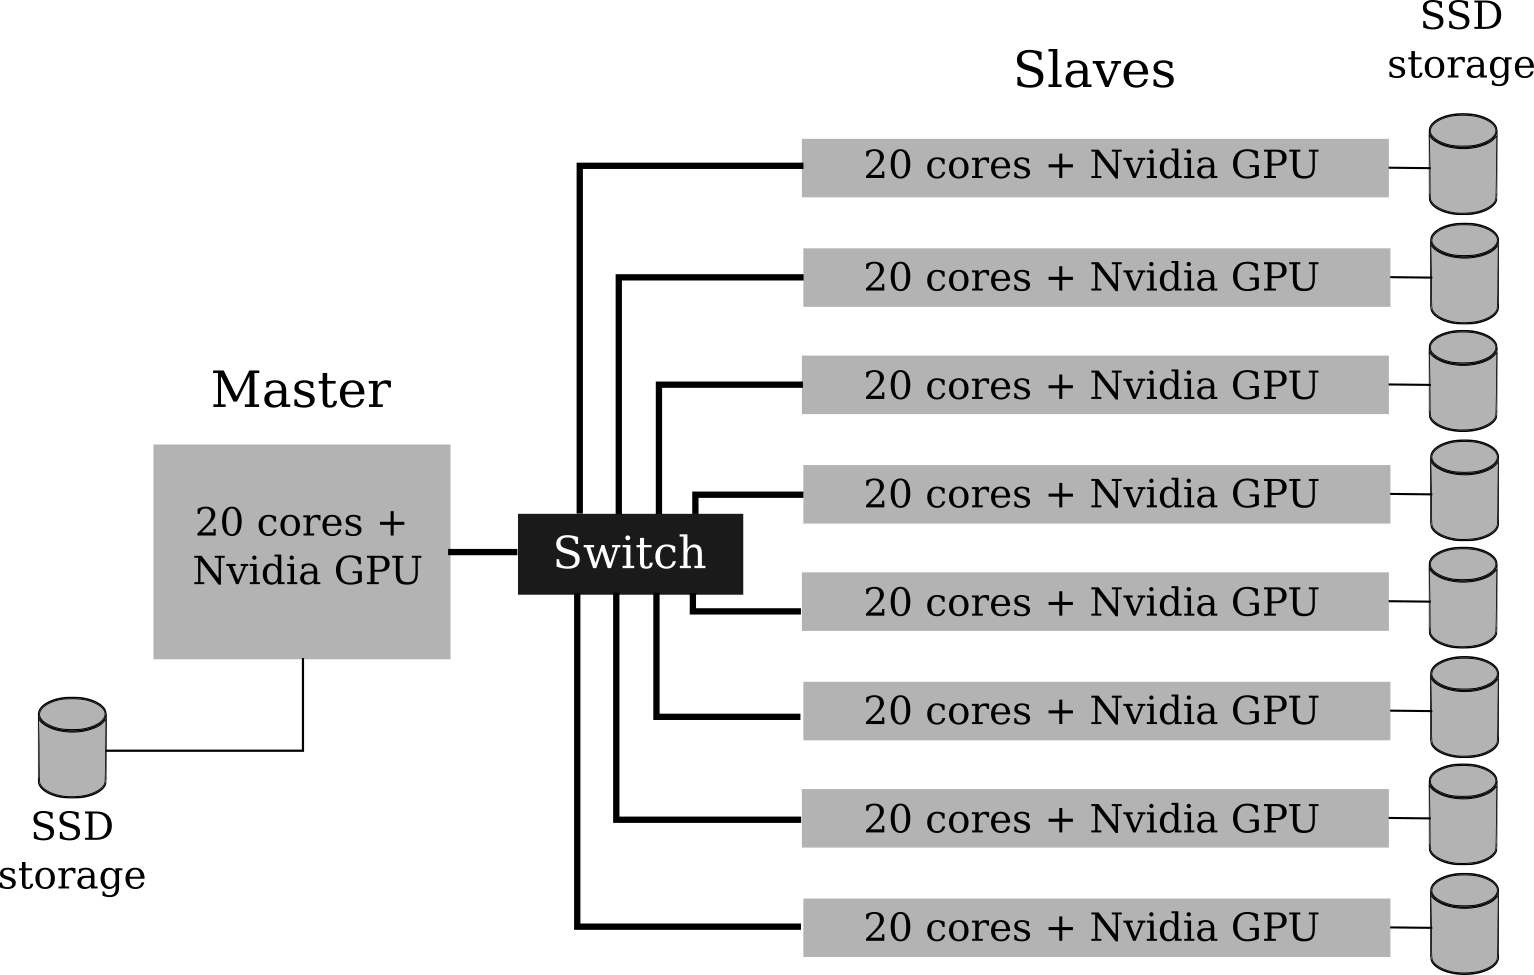
\includegraphics[scale=0.7]{images/cluster-topologico.png}
  \caption{Cluster hardware.}
  \label{fig:cluster}
\end{figure}

The \textit{slave} machines are Dell workstations Precision R7910. These machines are equipped
with Dual Intel{\textregistered} Xeon{\textregistered} processors E5-2640 operating at $2.4$GHz with
$32$Gb of RAM each. They have 2x$10$GbE (Gigabit Ethernet) and 2x$1$Gbit network connectors, which
allow the use of the Gigabit network exclusively for intra-cluster communication. Each node
has a $360$Gb solid state disk for storage.

These equipments are also installed with Nvidia{\textregistered} GPUs (Graphic Processing Units) M4000{\textregistered} with $8$Gb CUDA\cite{CUDA} capable.
The GPUs on nodes, despite capable of visualization, are expected to be used as secondary calculation units.
The use of graphic processors for calculations is widely applied in scientific computing and these divides
are also called accelerators\cite{accelerators}.

The \textit{master} machine is a Dell Precision T7910, with very similar configuration of the slaves. The main
differences rely on the graphics processor unit, equipped with another Nvidia{\textregistered} GPU: a
Quadro{\textregistered} M2000 with $4$Gb of memory. These video card is not aimed for calculations, but for
visualization of data and graphics display. The other different is in the main RAM memory, having the \textit{master}
$256$Gb of RAM. 

A set of three hard-disks of $500$Gb was installed to the master node, making an extra $1.5$Tb to be used as part
of the distributed file system.

The original OS sold with the cluster is an OEM (Original Equipment Manufacturer) Windows 7{\textregistered}\cite{windows7}. This
OS is not supported by the whole set of software expected to be used by the research group users. The chosen
system to replace the original Windows 7 is CentOS (Community Enterprise Operating System)\cite{centos}, which offers a platform to natively run all
software needed by the users. CentOS is a community driven free-software effort which focuses in provide a robust open source ecosystem.
Its typical users are organizations or individuals which have professional oriented hardware but do not need strong commercial support
in order to achieve successful operation. It is fully compatible with Red Hat Enterprise Linux and in full compliance with Red Hat's
redistribution requirements.

Details on possible options for software compatibility and operating system independence will be given on subsections \ref{ssub:dock} and \ref{ssub:virt}

%------------------------------------------------------------------------------
\subsection{Linux Operating System}

The reason for choosing \textit{CentOS} as the Linux flavor for the system is due to its characteristics and the previous
experience of the cluster management team. CentOS is aimed to offer a free, enterprise-class, community-supported computing
functionality. It appeared as a fork of Red Hat Enterprise Linux, which is available only trough paid subscription. The option
for CentOS, in this context, is to have both the strong development for enterprise systems and also its gratuity.

A second reason is to take advantage of previous competence of the installation and user team which already has experience
in using Fedora Linux, a distribution fully compatible with CentOS.

That said, all the software currently in use by the Thermal-Hydraulics Laboratory team are compatible with CentOS. This
makes this flavor of Linux the straightforward choice for the cluster system. It is also worth noting that the use of
free and open-source software has a social meaning in promoting the share of knowledge.

%------------------------------------------------------------------------------
\subsection{Software Solutions}
\label{sub:ssol}

Before choosing a software for perform a desirable task, its mandatory to have a consistent definition of the environment
in which the system will be used. The first constraint is the network environment. It's worth noting that the cluster is
located in the CDTN network and the restrictions and security rules enforced in the network must be followed by the system.

With this is mind, the choice is to have the main system - interchangeably called slave machines or cluster nodes - in one isolated sub-network only accessed by
the master node. The master node is part of both the sub-network and the institute's network. The sole point of access to the
internet for any slave is the master node which, in turn, is connected to the internet using a proxy connection and a
NAT (Network Access Translation). The topology of the cluster network is presented in Figure~\ref{fig:esquema-cluster}.

\begin{figure}[h] % t forces top and b forces bottom: can be added to h, ex. [ht]
%  \centering\includegraphics[width=8.5cm,height=8.5cm]{images/esquema_cluster_edited_bw.png}
  \centering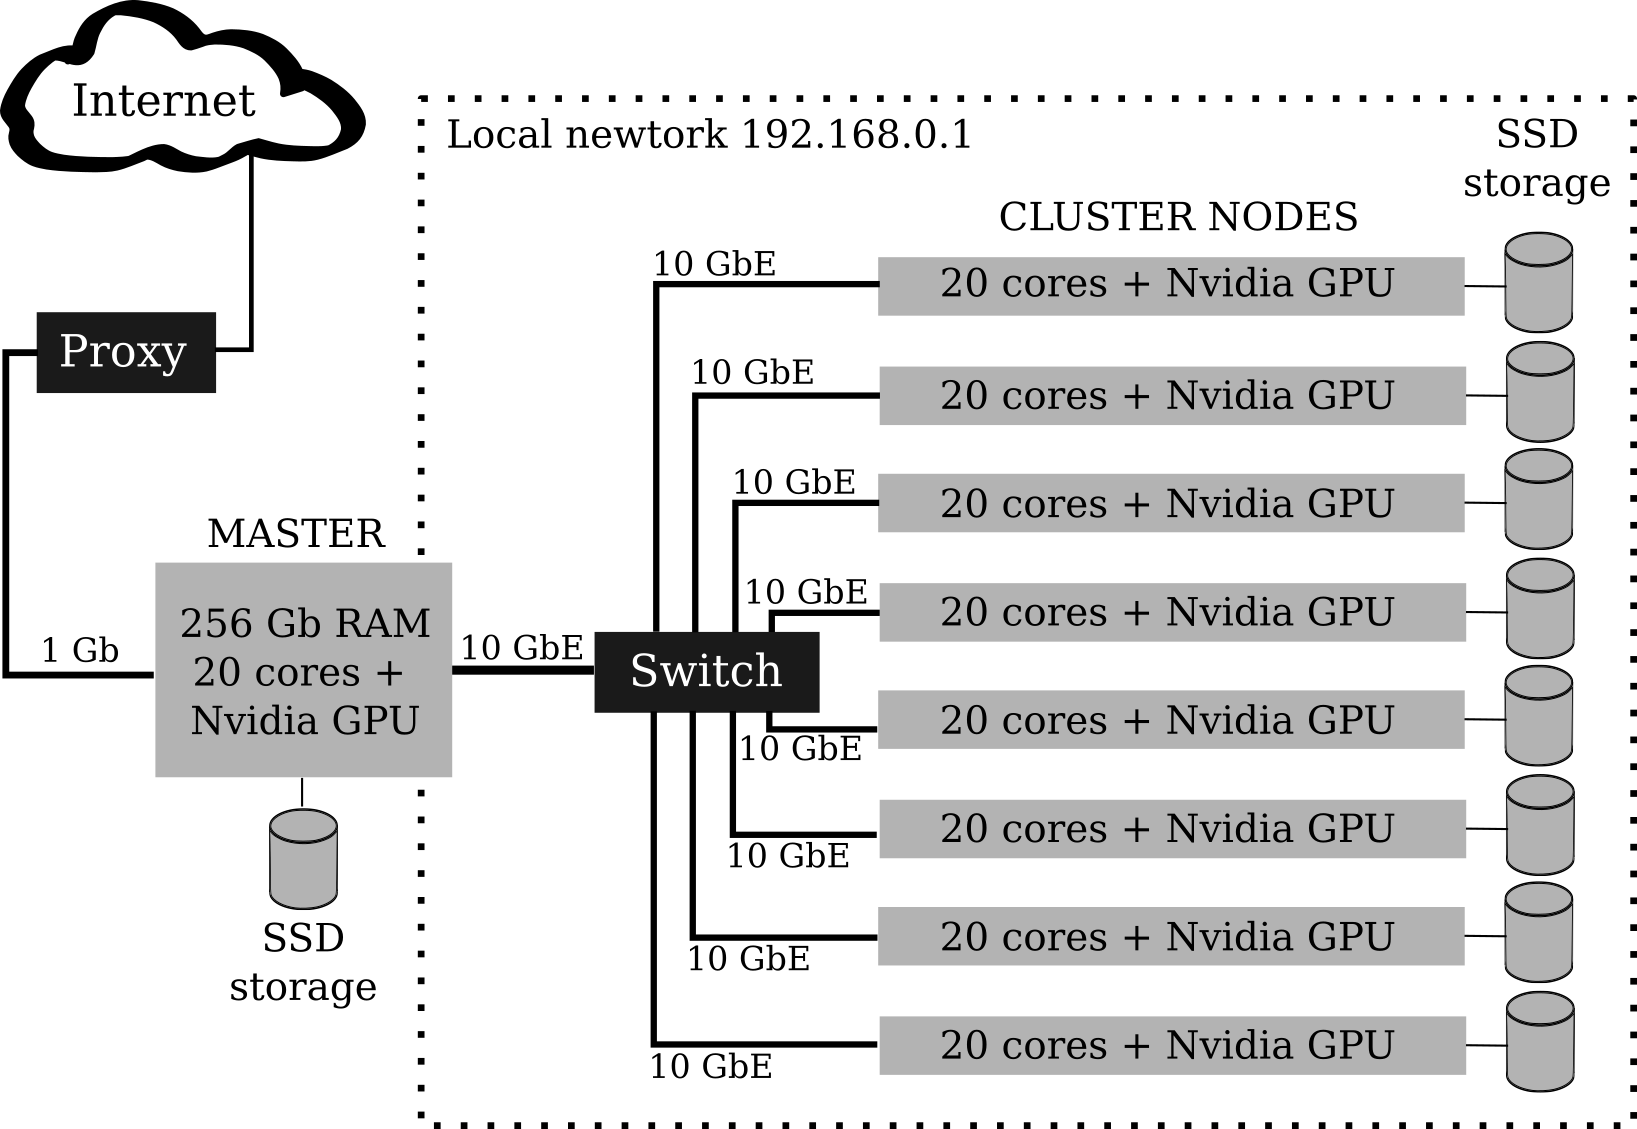
\includegraphics[scale=0.7]{images/cluster-rede.png}
  \caption{Cluster showing its network topology.}
  \label{fig:esquema-cluster}
\end{figure}

The chosen network topology have impacts on system maintenance. Since the slave machines cannot access the internet, the
master is configured to hold a mirror of packages installed in all system machines. The average download rate for main CentOS package provider site at the
master node is of $500$Kbytes/second in trough the proxy in CDTN's network.
With this in mind, the master machine is scheduled to make updates from time to time (once a week in the current configuration) while the slaves are also scheduled to
make their updates after the master and from master's local repository. This approach has advantages, like decreasing internet bandwidth demand since only
one machine downloads updated packages from the internet. Other advantage is in downloading time, since the slaves
use dedicated $10$GbE connections to the master which provides the necessary packages.

As expected, this approach has its drawback. A certain amount of disk space is needed to keep a mirror of CentOS packages locally.
To decrease this space consumption, only packages already installed on the system - master and slaves - are
downloaded and kept in the local repository. In the case of the installation of a new package not yet present in the repository,
it must be installed in the master. After that, the scheduled script guarantees its availability for the slaves. In the uncommon
situation where a package is necessary for the nodes but not for the master, it must be manually added to the repository. This task
is facilitated by CentOS packages manager \verb yum \cite{yum}

However, there are more than one way of setup a cluster system with respect
to file system, software execution and user access.

The next sub-sections describe alternatives to the use of a direct installation of CentOS version of Linux operating system.
They are not currently in use in the describe cluster system, but are presented in this paper as they remain as alternatives
or complementary options for specific cases. For example, the use of a software which is incompatible with another one already
in use.

%------------------------------------------------------------------------------
\subsubsection{Docker}
\label{ssub:dock}

Docker is a software technology providing containers. A container can be seen as an isolated user space provided by the operating system
kernel. Docker technology works providing an additional level of abstraction and automation at operating system level. In other words,
docker provides a way of programs run without direct communication with the operating system. This makes programs unaware of details of the
system and less dependent on specific configurations of the operating system. Docker provides the middle-ware which controls the interaction
between programs and operating system.

Moreover, Docker allows applications to be efficiently distributed and executed in a portable manner. The same application can be easily
run in a wide range of computer platforms\cite{Boettiger}.

From the point of view of program developers, distribute their application as a Docker package avoids software installation and
setup procedures in the host machine. The toolchain complexity is performed only once in the Docker package. The system administrators,
on the other hand, only have to install Docker and its packages. No extra work to make applications run. A valuable and detailed evaluation
of the use of Docker in the high demand computational field of research of bioinformatics is presented by Tommaso et al.\cite{Tommaso}.

%------------------------------------------------------------------------------
\subsubsection{Operating System Virtualization}
\label{ssub:virt}

Virtualization is the creation and use of a version of (usually) an operating system inside another operating system. Virtualization
is a technique widely used for cloud computing, where users send their jobs to be running in non-local computers usually provided
as services. Virtualization makes possible to have many different machines installed following the needs of the users without the
problem of machines management. The main drawback of its use is that virtualization is costly in terms of performance, since operating system
resources that otherwise would be shared by many processes must be kept individually for each virtual machine.

There are solid studies on the use of virtualization as service for scientific research\cite{vir1,vir2}. In the present case, virtualization
is seen as a last resource for running essential software in the cases where the usual operating system or Docker do not work.

%------------------------------------------------------------------------------
\subsection{File System}

A crucial element of a computer system architecture is its file system. A file system is the set of data structures and functions an operating system
use to manage and keep track of files on disks and partitions. There is a large number of file systems being used by different operating systems\cite{linuxbook}.

However, in a high performance and high demand system like a cluster, there are some desirable features not usually provided for standard computers file systems.
For example, the ability to have many different interconnected computers reading and writing information concurrently and asynchronously. These kind of feature
is provided by a specialized file system, usually called distributed file system\cite{hal}.

The chosen solution for distributed file system management is the GlusterFS\cite{gluster}. GlusterFS is an open source, distributed file system and has
a unique no-metadata server architecture. Most distributed file systems use a metadata server, which has information on where to retrieve data which is
physically scattered among different disks. This architecture imposes a dependence on the metadata server. If it goes down, the system becomes inaccessible.
GlusterFS keeps this information as distributed hashes, avoiding the dependence on one server or node.

The control of Gluster is transparent for users, providing a level of abstraction with no impact on how users of the system operate with their files. This
abstraction also has no impact in system management. An envisaged quota control of user accounts can work without any problem above the GlusterFS file system.

Another option under consideration is the more robust Lustre file system\cite{lustre}. Lustre is a parallel distributed file system widely used in large-scale
cluster systems. Despite its reliability and recognized performance (high I/O throughput: more than a terabyte per second), it is not the first choice
for the distributed file system for the presented cluster due to its higher learning curve for installation and administration compared to GlusterFS.
It is important to keep in mind that as the cluster management personal is limited and formed by non-experienced system
administrators thus simpler systems are favored as long as they meet the operating criteria. The size of the presented cluster is also small by Lustre standards.

With that in mind, Lustre remains as a second option in the case of GlusterFS does not perform as expected. 

%------------------------------------------------------------------------------
\subsection{Visualization}

The presence of powerful GPU devices in each node of the cluster make possible their use for calculations. However,
this hardware can be used for its natural task: visualization. At a first glance, this can sound natural and
straightforward. However, there are trick details in using different nodes to render and output one image. The first one
is the ability to gather scattered information in order to produce the desirable output in one display.

Gladly, there is software aimed to data visualization which address the presented issue. Developed to be able to work with complex data,
Paraview\cite{paraview} is an open-source multiple-platform application for scientific visualization. Its design considers
the use of a client-server architecture in order to deal with data-sets scattered among many nodes in a multiprocessing
system. 


%------------------------------------------------------------------------------
\subsection{Graphics Processors: Extended Use}

The system under consideration has powerful GPU cards installed in machines
which have no output display. The use of GPUs to perform tasks other than graphics processing
is nowadays widespread in many fields of research \cite{gpgpu}. Modern software is written with
the objective of taking advantage of this ``extra'' processing capabilities and studies of software
engineering on parallelization of sequential algorithms to be applied in GPUs are a significant
nowadays.

In order to make the use of GPUs for general processing less difficult, libraries, compilers and
frameworks were developed. At the beginning these tools were developed and deployed by graphics cards
manufacturers. The pioneer in offering both GPUs cards capable of general use is Nvidia, which,
without surprise, is also pioneer in making a available a full framework for its GPU programming.
This tool is called CUDA (Compute Unified Device Architecture) and is the standard parallel computing platform
and application programming interface (API) model for Nvidia's graphic cards.

CUDA can be used together with many libraries for a wide range of programming tasks. Nvidia provides CUDA
auxiliary libraries for, for example, linear solvers (AmgX), deep neural networks (cuDNN), Fast Fourier Transform (cuFFT) and
many others. 

However, with the increase of the use the cards, developers start to demand some
standardization in order to be able experiment new algorithms in different cards. Today, the
reference framework for development for heterogeneous platforms is \textit{OpenCL}\cite{opencl}.

OpenCL\texttrademark (Open Computing Language) is an industry standard for task-parallel and
data-parallel heterogeneous computing. It is designed to work on a variety of modern
CPUs, GPUs, DSPs and other microprocessor designs. OpenCL provides a abstractions and a
programming API (Application Programming Interface) and defines a core functionality that all
devices must support, as well as optional functionality for high-function devices. It also
includes an extension mechanism that let vendors implement unique hardware features and
experimental programming interfaces for their devices and for the application developers
benefit. OpenCL does guarantee compatibility and portability at the expense of some less
of performance when compared to proprietary implementations.

The idea for the presented cluster system, is to provide both CUDA libraries for
software developed for Nvidia graphic cards and also OpenCL libraries to
be used by software written to make use of the programming genericity
provided by OpenCL. As the time of writing, the libraries were installed
in only one node of the cluster and tests are being envisaged to check
compatibility of both frameworks.

%------------------------------------------------------------------------------

\section{RESULTS AND ANALYSIS}

All the results presented in this section include the master node and only one slave node.
Since all slaves have identical hardware, it is sufficient to install and configure only one
node and after finishing, replicate a mirror of its configuration to other nodes\footnote{Few configurations like
  network IPs must be unique and thus configured after mirroring. However, this kind of task is simple enough to worth the mirroring approach.}
The current status of the system is that it is partially operational with some goals reached:

\begin{itemize}

\item Distributed file system GlusterFS up and running;
\item Master node installed and running with local packages repository up and running;
\item NVidia GPU drivers installed in the master node replacing the generic drivers provided by CentOS.
  
\end{itemize}

The short list above encompasses the very main steps to have the system running. All the next
steps can be seen as applications installation and fine tuning of the system configuration.
Some of the following steps are:

\begin{itemize}
\item Check the compatibility of Nvidia proprietary drivers already for the accelerators in the slave node with OpenCL implementation driver for the GPU;
\item Chose and install a reliable backup system for user accounts and define procedures for system configuration backup;
\item Define and install a user queue manager to control user precedence and access to nodes;
\item Install and test all scientific software to be used in the beginning of cluster operations.
\end{itemize}

In order to be able to verify the operation of the cluster, a list of elements of operation is under consideration.
This list is aimed to be a guide of what aspects are being complied with or not. The main idea is to have a score for
each operational aspect related to the system design (file system, user processes, disk occupancy, etc.) and after three, six and twelve months of full operation, be able to evaluate if the system is currently
operating satisfactorily.

%------------------------------------------------------------------------------

\section{CONCLUSIONS AND PERSPECTIVES}

%(O que está bom, o que está ruim na atual instalação)
%(Trabalhos futuros: pra onde ir (operação), possíveis mudanças)

The process of acquiring, installing and managing a cluster system is a very specific task aimed to well trained
personal. In a perfect situation, a team of specialists would take care of these tasks letting the users - scientists in the present case -
free to focus on their research work and on how to take the most of such system. However, in other cases the users themselves must
take care of the whole process.

Although challenging, this can be seen as an opportunity to have a deeper of understanding of the tool one must use the accomplish his tasks.
This the case in this work, where the users had to chose among many options to make a professional cluster operational.

As an ongoing work, some of the challenges - like defining and installing a distributed file system, for example - were successfully
addressed. Other remain to be figured out and worked out.

There are many ongoing tasks and even more tasks still to be started. To mention a few, one
interesting task related to the reliability and data management is the implementation of
a automatic process of shutdown on loss of power supply. Other one is to define a systematic
user account backup to avoid loss of data of expensive simulations at the same time ensuring
disk space availability.

As a conclusion, there is a clear trade-off between the situation where the tool - at the limit, a complex tool like a cluster is a tool - is available and ready to use and
the discussed case in this paper. The former clearly saves precious time that scientists can devote to their research work itself. However, the latter situation has a not so obvious
advantage: being forced to expend time to understand details of the cluster operation, scientists can acquire a new perspective on how to apply their
methods. This can lead to changes or improvements in the way a problem is solved. If this is a real advantage is yet to be shown. However,
in a situation like the one presented, where there is no choice, this can be seen as a positive condition on the improvement of methods, solutions and approaches used
uncritically on a daily basis.


%Uma cita\c{c}\~{a}o \cite{Henderson17}.


%------------------------------------------------------------------------------



\section*{Acknowledgments}
The authors would like to thank FUJB for financing the cluster acquisition
as part of the project \textit{Desenvolvimento de novos elementos combust\'{i}veis nucleares
  e materiais e pe\c{c}as para combust\'{i}veis nucleares}, agreement FINEP 01.07.0548.00 - Process FUJB 13.867-3.
The authors also thank Dr. Jo\~{a}o Roberto Loureiro de Mattos for the work which made possible the acquisition
of the cluster.

%%%%%%%%%%%%%%%%%%%%%%%%%%%%%%%%%%%%%%%%%%%%%%%%%%%%%%%%%%%%%%%%%%%%%%%%%%%%%%%%%%%%%%%%%%%%

\begin{thebibliography}{99} %99 é o número máximo que o thebibliography permite. Numero de referencias que aparecerão.

\bibitem{linux} ``The Linux Documentation Project'', \\\verb#http://www.tldp.org/LDP/intro-linux/html/chap_01.html# (2017).

\bibitem{Dongarra2017} John Dongarra et. al., ``With Extreme Computing, the Rules Have Changed'', \textit{Computing in Science Engineering}, \textbf{19}, pp. 52--62, (2017).

\bibitem{CUDA} John Nickolls, Ian Buck, Michael Garland and Kevin Skadron, ``Scalable Parallel Programming with CUDA'', \textit{Queue - GPU Computing}, \textbf{6}, pp. 40--53, (2008).

\bibitem{accelerators} ``What is GPU-accelerated computing?'', \\\verb#http://www.nvidia.com/object/what-is-gpu-computing.html# (2017).

\bibitem{windows7} Jorge Orchilles, \textit{Microsoft Windows 7 Administrator's Reference}, Syngress, Boston USA (2010).
  
  % Centos
\bibitem{centos} ``The CentOS Project'', \verb#https://www.centos.org# (2017).

\bibitem{yum} ``man7.org yum man page'', \verb#http://man7.org/linux/man-pages/man8/yum.8.html# (2017).
  
\bibitem{Boettiger} Carl Boettiger, ``An introduction to Docker for reproducible research'', \textit{SIGOPS Operating System Review}, \textbf{49}, pp. 71--79, (2015).

\bibitem{Tommaso} Paolo Di Tommaso et al. ``The Impact of Docker Containers on the Performance of Genomic Pipelines'' \textit{PeerJ}, \textbf{3}, (2015).

  % Virtualizacao (9 e 10)
\bibitem{vir1} A. J. Younge and G. C. Fox, ``Advanced Virtualization Techniques for High Performance Cloud Cyberinfrastructure'', \textit{2014 14th IEEE/ACM International Symposium on Cluster, Cloud and Grid Computing}, Chicago, IL, USA, pp. 583--586, May, (2014).
  
\bibitem{vir2} I. Sadooghi, J. H. Martin, T. Li, K. Brandstatter, K. Maheshwari, T. P. P. de Lacerda Ruivo, G. Garzoglio, S. Timm, Y. Zhao and I. Raicu, ``Understanding the Performance and Potential of Cloud Computing for Scientific Applications'', \textit{IEEE Transactions on Cloud Computing}, \textbf{5}, pp. 358--371, (2017).
  
\bibitem{linuxbook} Wirzenius and Lars, \textit{The  Linux System Administrator's Guide}, iUniverse incorporated (2000).

\bibitem{hal} Benjamin Depardon, Ga\"{e}l Le Mahec and Cyril S\'{e}guin, ``Analysis of Six Distributed File Systems'', Research Report, pp. 44, (2013).
  
\bibitem{gluster} Alex Davies and Alessandro Orsaria, ``Scale out with GlusterFS'', \textit{The Linux Journal}, \textbf{2013}, (2013).

\bibitem{lustre} ``Lustre* Software Release 2.x: Operations Manual'', Editor: Intel Corporation, (2017).

\bibitem{paraview} Ayachit, Utkarsh, \textit{The ParaView Guide: A Parallel Visualization Application}, Kitware, ISBN 978-1930934306, (2015).

  \bibitem{gpgpu}  John D. Owens, David Luebke, Naga Govindaraju, Mark Harris, Jens Kr\"{u}ger, Aaron E. Lefohn, and Tim Purcell, ``A Survey of General-Purpose Computation on Graphics Hardware'', \textit{Computer Graphics Forum}, \textbf{26(1)}, pp. 80--113, March (2007).

  \bibitem{opencl} J. E. Stone, D. Gohara and G. Shi, ``OpenCL: A Parallel Programming Standard for Heterogeneous Computing Systems'', \textit{Computing in Science \& Engineering}, \textbf{12(3)}, pp. 66--73, May-June (2010).

\end{thebibliography}

% ---------------------------------------------------------
% Minha bibliografia usando arquivo externo
%\bibliographystyle{unsrt}
%\bibliography{bibli}


\end{document}
